%\documentclass{klausur}
\documentclass[answers]{klausur}

\setlength{\hoffset}{-0.7cm}
\setlength{\textwidth}{17.cm}
\setlength{\oddsidemargin}{0pt}
\setlength{\evensidemargin}{0pt}
\setlength{\parindent}{0em}
\setlength{\voffset}{-2.cm}
\setlength{\headheight}{120pt}
\pagestyle{headandfoot}

\renewcommand{\solutiontitle}{\noindent\textbf{Lösung:}\par\noindent}

\begin{document}

	% Parameters: Name of exam, Semester
	\setExamHeaderAndFooter{Beck/Protogerakis}{Klausur Fach ABC (11031)}{WiSe 2024/25}
	
	% Parameters: Name of exam, Semester, Date, Time, Result table (depending on number of problems)
	\makeExamTitlePage{Klausur Fach ABC (11031)}{WiSe 2024/25}{24.01.2025}{10:30 - 12:00}{
	{\large 
		\gradetable[h][questions]
	}}{Prof. Dr.-Ing. Beck/Prof. Dr.-Ing. M. Protogerakis}
	
	% Parameters: Duration of exam, number of problems, number of pages, number of allowed hand-written pages
	
	\makeExamRulesPage{90}{\numquestions}{\numpages}{2}
	
	\newpage

{\Large\bf Formelsammlung}
\vskip 24pt
{\large\bf Korrespondenztabelle Laplace-Transformation}
\vskip 12pt

\begin{tabularx}{\textwidth}{|p{11cm}|X|} 
	\hline
	&\\
	\(f(t)\) für \(t\ge 0\) & \multirow{2}{*}{\(F(s)\)} \\
	\(f(t)=0\) für \(t<0\) & \\
	&\\
	\hline
	\hline
	&\\
	\(\delta(t)\) & 1 \\
	&\\
	\hline
	&\\
	\(\delta(t-T_t)\) & \(e^{-sT_t}\) \\
	&\\
	\hline
	&\\
	\(\sigma(t)\) & \(\frac{1}{s}\)\\
	&\\
	\hline
	&\\
	\(t\) & \(\frac{1}{s^2}\)\\
	&\\
	\hline
	&\\
	\(\frac{1}{2}\cdot t^2\) & \(\frac{1}{s^3}\)\\
	&\\
	\hline
	&\\
	\(\frac{1}{n!}\cdot t^n\) & \(\frac{1}{s^{n+1}}\)\\
	&\\
	\hline
	&\\
	\(e^{at}\) & \(\frac{1}{s-a}\)\\
	&\\
	\hline
	&\\
	\(\frac{1}{T}\cdot e^{-t/T}\) & \(\frac{1}{Ts+1}\) \\
	&\\
	\hline
	&\\
	\(1-e^{-t/T}\) & \(\frac{1}{s\cdot(Ts+1)}\) \\
	&\\
	\hline
	&\\
	\(\frac{1}{T}\cdot\left(\delta(t)-\frac{1}{T}\cdot e^{-t/T}\right)\) & \(\frac{s}{Ts+1}\) \\
	&\\
	\hline
	&\\
	\(\frac{T_1}{T_2}\cdot\delta(t)+\frac{T_2-T_1}{T_2^2} e^{-t/T_2}\) & \(\frac{T_1s+1}{T_2s+1}\)  \\
	&\\
	\hline
\end{tabularx}
\newpage

\begin{tabularx}{\textwidth}{|p{13.5cm}|X|} 
	\hline
	&\\
	\(f(t)\) für \(t\ge 0\) & \multirow{2}{*}{\(F(s)\)} \\
	\(f(t)=0\) für \(t<0\) & \\
	&\\
	\hline
	\hline
	&\\
	\(\frac{1}{T_1-T_2}\cdot\left(e^{-t/T_1}-e^{-t/T_2}\right),\qquad\qquad\qquad\qquad\qquad\qquad\qquad\qquad\qquad T_1\ne T_2\) & \(\frac{1}{\left(T_1s+1\right)\cdot\left(T_2s+1\right)}\) \\
	&\\
	\hline
	&\\
	\(1-\frac{1}{T_1-T_2}\cdot\left(T_1\cdot e^{-t/T_1}-T_2\cdot e^{-t/T_2}\right),\qquad\qquad\qquad\qquad\qquad\qquad\;\;\, T_1\ne T_2\) & \(\frac{1}{s\cdot\left(T_1s+1\right)\cdot\left(T_2s+1\right)}\) \\
	&\\
	\hline
	&\\
	\(\frac{1}{T_1\cdot T_2\cdot \left(T_1-T_2\right)}\cdot\left(T_1\cdot e^{-t/T_2}-T_2\cdot e^{-t/T_1}\right),\qquad\qquad\qquad\qquad\qquad\qquad T_1\ne T_2\) & \(\frac{s}{\left(T_1s+1\right)\cdot\left(T_2s+1\right)}\) \\
	&\\
	\hline
	&\\
	\(\frac{t}{T^2}\cdot e^{-t/T}\) & \(\frac{1}{(Ts+1)^2}\)  \\
	&\\
	\hline
	&\\
	\(1-e^{-t/T}\cdot\left(1+\frac{t}{T}\right)\) & \(\frac{1}{s(Ts+1)^2}\)  \\
	&\\
	\hline
	&\\
	\(e^{-t/T}\cdot\left(\frac{1}{T^2}-\frac{t}{T^3}\right)\) & \(\frac{s}{(Ts+1)^2}\)  \\
	&\\
	\hline
	&\\
	\(\frac{\omega_0}{\sqrt{1-D^2}}\cdot e^{-D\omega_0 t}\cdot\sin\left(\omega_D t\right),\qquad\qquad\qquad\qquad\quad |D|<1,\;\omega_D=\omega_0\cdot\sqrt{1-D^2}\) & \(\frac{\omega_0^2}{s^2+2D\omega_0\cdot s+\omega_0^2}\) \\
	&\\
	\hline
	&\\
	\(1-e^{-D\omega_0 t}\cdot\left(\cos\left(\omega_D t\right)+\frac{D}{\sqrt{1-D^2}}\cdot\sin\left(\omega_D t\right)\right),\quad |D|<1,\;\omega_D=\omega_0\cdot\sqrt{1-D^2}\) & \(\frac{\omega_0^2}{s\cdot\left(s^2+2D\omega_0\cdot s+\omega_0^2\right)}\) \\
	&\\
	\hline
	&\\
	\(\omega_0^2\cdot e^{-D\omega_0 t}\cdot\left(\cos\left(\omega_D t\right)-\frac{D}{\sqrt{1-D^2}}\cdot\sin\left(\omega_D t\right)\right),\quad |D|<1,\;\omega_D=\omega_0\cdot\sqrt{1-D^2}\) & \(\frac{s\cdot\omega_0^2}{s^2+2D\omega_0\cdot s+\omega_0^2}\) \\
	&\\
	\hline
	&\\
	\(\frac{t^{n-1}}{(n-1)!\cdot T^n}\cdot e^{-t/T}\) & \(\frac{1}{(Ts+1)^n}\) \\
	&\\
	\hline
	&\\
	\(1- e^{-t/T}\cdot\sum_{k=0}^{n-1}\frac{t^k}{T^k\cdot k!}\) & \(\frac{1}{s(Ts+1)^n}\) \\
	&\\
	\hline
\end{tabularx}
\newpage

\begin{tabularx}{\textwidth}{|p{11cm}|X|} 
	\hline
	&\\
	\(f(t)\) für \(t\ge 0\) & \multirow{2}{*}{\(F(s)\)} \\
	\(f(t)=0\) für \(t<0\) & \\
	&\\
	\hline
	\hline
	&\\
	\(\sin\left(\omega t\right)\) & \(\frac{\omega}{s^2+\omega^2}\) \\
	&\\
	\hline
	&\\
	\(\sin\left(\omega t+\varphi\right)\) & \(\frac{s\cdot\sin\varphi+\omega\cdot\cos\varphi}{s^2+\omega^2}\) \\
	&\\
	\hline
	&\\
	\(t\cdot\sin\left(\omega t\right)\) & \(\frac{2\omega s}{\left(s^2+\omega^2\right)^2}\) \\
	&\\
	\hline
	&\\
	\(t^n\cdot\sin\left(\omega t\right)\) & \(j\frac{n!}{2}\cdot\left(\frac{1}{(s+j\omega)^{n+1}}-\frac{1}{(s-j\omega)^{n+1}}\right)\) \\
	&\\
	\hline
	&\\
	\(e^{at}\cdot\sin\left(\omega t\right)\) & \(\frac{\omega}{(s-a)^2+\omega^2}\) \\
	&\\
	\hline
	&\\
	\(\sinh\left(\omega t\right)\) & \(\frac{\omega}{s^2-\omega^2}\) \\
	&\\
	\hline
	&\\
	\(\cos\left(\omega t\right)\) & \(\frac{s}{s^2+\omega^2}\) \\
	&\\
	\hline
	&\\
	\(\cos\left(\omega t+\varphi\right)\) & \(\frac{s\cdot\cos\varphi-\omega\cdot\sin\varphi}{s^2+\omega^2}\) \\
	&\\
	\hline
	&\\
	\(t\cdot\cos\left(\omega t\right)\) & \(\frac{s^2-\omega^2}{\left(s^2+\omega^2\right)^2}\) \\
	&\\
	\hline
	&\\
	\(t^n\cdot\cos\left(\omega t\right)\) & \(\frac{n!}{2}\cdot\left(\frac{1}{(s+j\omega)^{n+1}}-\frac{1}{(s-j\omega)^{n+1}}\right)\) \\
	&\\
	\hline
	&\\
	\(e^{at}\cdot\cos\left(\omega t\right)\) & \(\frac{s-a}{(s-a)^2+\omega^2}\) \\
	&\\
	\hline
	&\\
	\(\cosh\left(\omega t\right)\) & \(\frac{s}{s^2-\omega^2}\) \\
	&\\
	\hline
\end{tabularx}
\newpage

\begin{tabularx}{\textwidth}{|p{11cm}|X|} 
	\hline
	&\\
	\(f(t)\) für \(t\ge 0\) & \multirow{2}{*}{\(F(s)\)} \\
	\(f(t)=0\) für \(t<0\) & \\
	&\\
	\hline
	\hline
	&\\
	\(1-\cos\left(\omega t\right)\) & \(\frac{\omega^2}{s\left(s^2+\omega^2\right)}\) \\
	&\\
	\hline
	&\\
	\(\omega t-\sin\left(\omega t\right)\) & \(\frac{\omega^3}{s^2\left(s^2+\omega^2\right)}\) \\
	&\\
	\hline
	&\\
	\(\sin\left(\omega t\right)-\omega t\cdot\cos\left(\omega t\right)\) & \(\frac{2\omega^3}{\left(s^2+\omega^2\right)^2}\) \\
	&\\
	\hline
	&\\
	\(\sin\left(\omega t\right)+\omega t\cdot\cos\left(\omega t\right)\) & \(\frac{2\omega s^2}{\left(s^2+\omega^2\right)^2}\) \\
	&\\
	\hline
\end{tabularx}

\vspace{2cm}
{\large\bf Formelsammlung zur Einführung in die Leitungstheorie}


\[
\begin{pmatrix}
	\underline U(l) \\
	\underline I(l) \\
\end{pmatrix}
=
\begin{pmatrix}
	\cosh(\underline \gamma \, l) & \underline Z_W \cdot \sinh(\underline \gamma \, l) \\
	\frac{\sinh(\underline \gamma \, l)}{\underline Z_W} & \cosh(\underline \gamma \, l) \\
\end{pmatrix}
\cdot
\begin{pmatrix}
	\underline U(l=0) \\
	\underline I(l=0) \\
\end{pmatrix}
\]
mit
\[\underline \gamma=\sqrt{(R' + \mathrm{j}\omega L')\cdot(G' + \mathrm{j}\omega C')}=\alpha+\mathrm{j} \, \beta\]
\begin{eqnarray*}
	\sinh(\mathrm{j} \, \beta \, l) = \mathrm{j} \cdot \sin( \, \beta \, l) & \mathrm{und} &\cosh(\mathrm{j} \, \beta \, l) =  \cos( \, \beta \, l) \\
\end{eqnarray*}
\[\underline U(z)= \underline U_0^+ \mathrm{e}^{- \mathrm{j} \underline \gamma \, z} + \underline U_0^- \mathrm{e}^{+ \mathrm{j}\underline \gamma \, z}\]
\[\underline I(z)=  \frac{\underline U_0^+}{ \underline Z_0} \mathrm{e}^{- \mathrm{j}\underline \gamma \, z} - \frac{\underline U_0^-}{ \underline Z_0} \mathrm{e}^{+ \mathrm{j}\underline \gamma \, z}\]
\[\underline Z_{Ltg}=\sqrt{\frac{R' + j\omega L'}{G' + j\omega C'}}\]


\begin{aufgaben}
		
\aufgabe[6]
Lorem ipsum dolor sit amet, consetetur sadipscing elitr, sed diam nonumy eirmod tempor invidunt ut labore et dolore magna aliquyam erat, sed diam voluptua. At vero eos et accusam et justo duo dolores et ea rebum. Stet clita kasd gubergren, no sea takimata sanctus est Lorem ipsum dolor sit amet. Lorem ipsum dolor sit amet, consetetur sadipscing elitr, sed diam nonumy eirmod tempor invidunt ut labore et dolore magna aliquyam erat, sed diam voluptua. At vero eos et accusam et justo duo dolores et ea rebum. Stet clita kasd gubergren, no sea takimata sanctus est Lorem ipsum dolor sit amet. Lorem ipsum dolor sit amet, consetetur sadipscing elitr, sed diam nonumy eirmod tempor invidunt ut labore et dolore magna aliquyam erat, sed diam voluptua. At vero eos et accusam et justo duo dolores et ea rebum. Stet clita kasd gubergren, no sea takimata sanctus est Lorem ipsum dolor sit amet. Lorem ipsum dolor sit amet, consetetur sadipscing elitr, sed diam nonumy eirmod tempor invidunt ut labore et dolore magna aliquyam erat, sed diam voluptua. At vero eos et accusam et justo duo dolores et ea rebum. Stet clita kasd gubergren, no sea takimata sanctus est Lorem ipsum dolor sit amet.

Lorem ipsum dolor sit amet, consetetur sadipscing elitr, sed diam nonumy eirmod tempor invidunt ut labore et dolore magna aliquyam erat, sed diam voluptua. At vero eos et accusam et justo duo dolores et ea rebum. Stet clita kasd gubergren, no sea takimata sanctus est Lorem ipsum dolor sit amet. Lorem ipsum dolor sit amet, consetetur sadipscing elitr, sed diam nonumy eirmod tempor invidunt ut labore et dolore magna aliquyam erat, sed diam voluptua. At vero eos et accusam et justo duo dolores et ea rebum. Stet clita kasd gubergren, no sea takimata sanctus est Lorem ipsum dolor sit amet.

\vskip 12pt
\begin{center}
	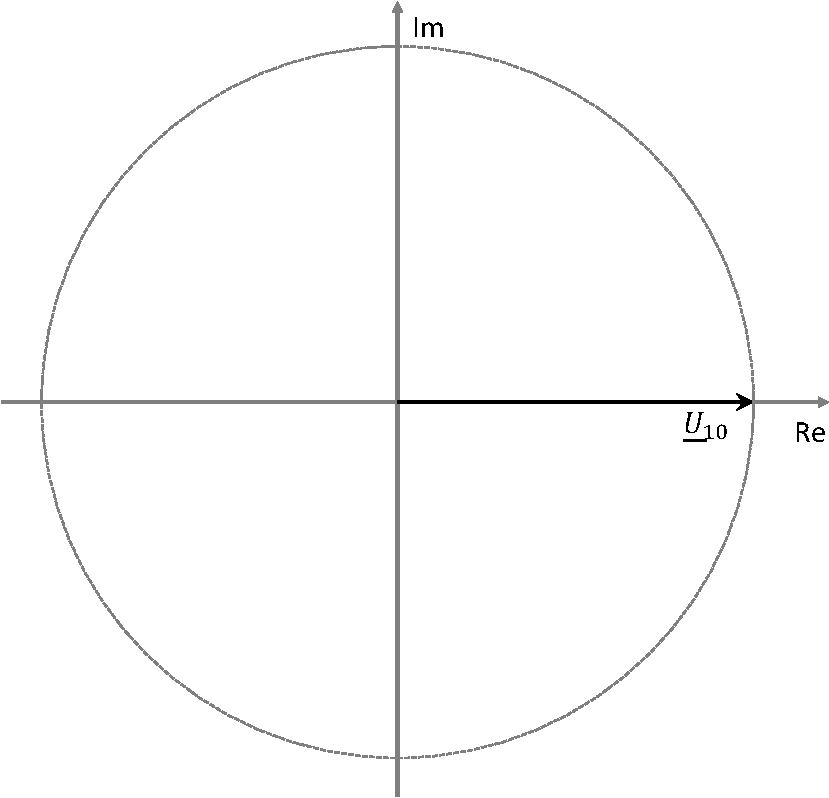
\includegraphics[width=13cm]{aufgabe_xyz/aufgabe4-crop}
\end{center}

\begin{solution}[15cm]
	\begin{center}
		\[ k = |\underline{U_{12}}|/|\underline{U_{10}}| = 2 \cdot \sin \left(\frac{\mathrm{\pi}}{m} \right)\]
	\end{center}
\end{solution}

\newpage
 
\end{aufgaben}
\end{document}

